\documentclass[11pt, oneside]{article}   	% use "amsart" instead of "article" for AMSLaTeX format
\usepackage{geometry}                		% See geometry.pdf to learn the layout options. There are lots.
\geometry{a4paper}
\usepackage[parfill]{parskip}    			% Activate to begin paragraphs with an empty line rather than an indent
%\usepackage{amssymb}
\usepackage{graphicx}
\usepackage{amsmath}
\usepackage{amssymb}
\graphicspath{ {images/} }

% For adding the headers
\usepackage{fancyhdr}
\pagestyle{fancy}
\fancyhf{}
    \setlength{\headheight}{14pt}
    \lhead{150023118}
    \chead{CS3302 Practical 2}
    \rhead{November 24, 2017}
    \rfoot{\thepage}

%\begin{verbatim}
%\end{verbatim}	
\usepackage{fancyvrb}

\usepackage{tikz}
\usetikzlibrary{matrix,decorations.pathreplacing}

\title{CS3302 Practical 2: Hamming Codes}
\author{150023118}
\date{November 24, 2017}

\begin{document}
\maketitle
\section*{Overview}

The objective of this practical was to implement Hamming codes and allow the user to experiment with Hamming codes through a GUI. The user was to be able to specify a number from 2 to 6 for parameter \textit{r} and encode words with the corresponding Hamming encoding. Additionally, the application corrupts codewords at a certain probability, which the parity-checker tries to correct. The user is able to experiment with different error rates and parameters. 

\section*{Usage}

This application requires Python 3 (tested on version 3.6.3). Additional dependencies can be installed using

\begin{Verbatim}[tabsize=4]
	$ pip3 install -r requirements.txt
\end{Verbatim}

After all dependencies have been set up, the application can be launched with:

\begin{Verbatim}[tabsize=4]
	$ cd hamming_app/
	$ python3 flask_app.py
\end{Verbatim}

Once the application is running, the main window should be accessible on any browser at http://127.0.0.1:8080. 
%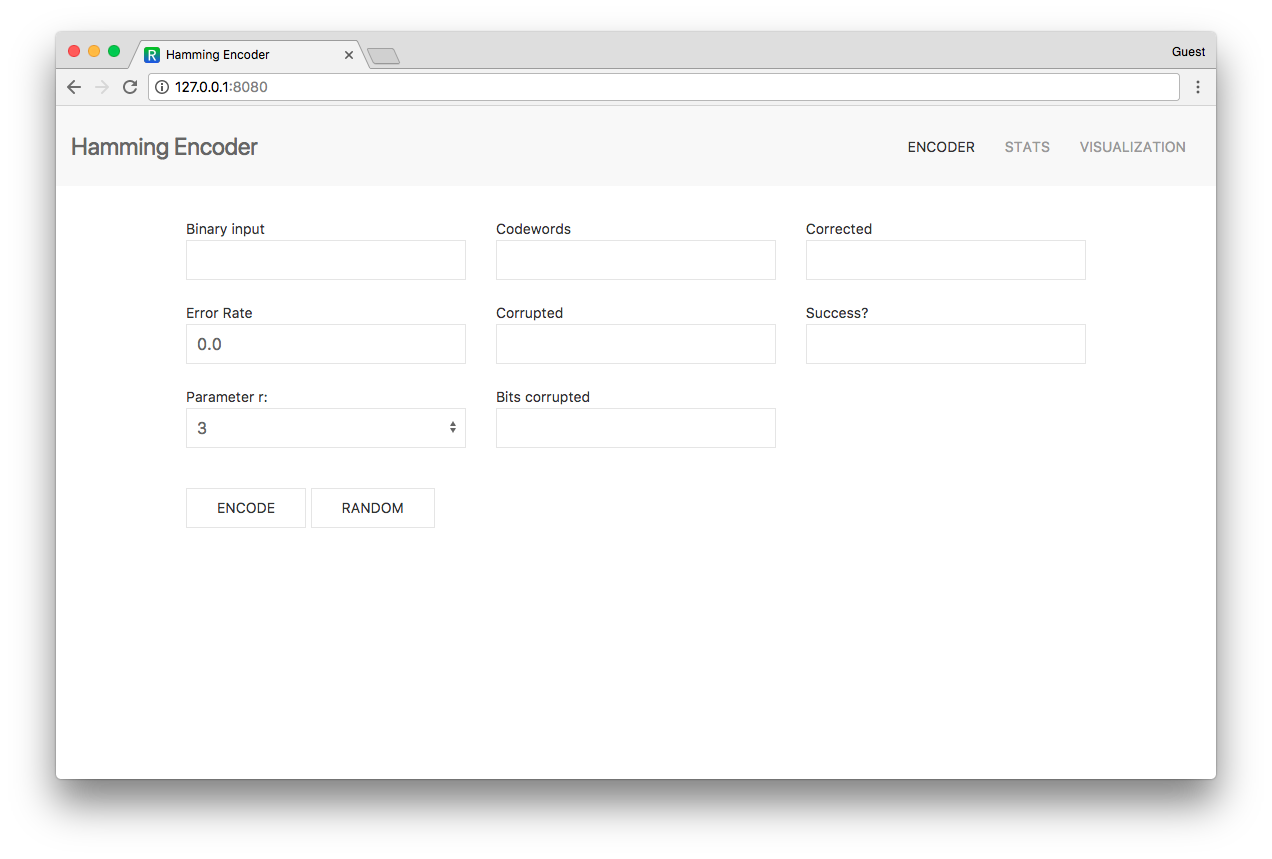
\includegraphics[width=\textwidth]{main_blank}

\section*{Design}

This application was written as a Python web application that delivered though Flask. The code for serving the pages is contained within \verb!flask_app.py!, and the classes for the Hamming encoder and checker are included in \verb!hammingclasses.py!. 

Instances of the class \verb|HammingEncoder| takes in a word and returns a codeword with the original bits in the word with parity bits attached. The constructor takes in the parameter \textit{r} as its argument and generates a Hamming encoder with a generator matrix. 

The generator matrix is configured so that the parity bits are as follows:

\begin{align*}
D &= \{\,i \mid \exists \, j \in \mathbb{N} \text{ such that } 2^j = i \ \& \ i < n \, \} &\\
P &= \{\,i \mid 1 \leq i \leq n \ \& \  i \notin D \}
\end{align*}


\section*{Testing}



\end{document}  